\documentclass[border=10pt,tikz]{standalone}
\usepackage{tikz}
\usetikzlibrary{positioning,arrows.meta,shapes}
\begin{document}
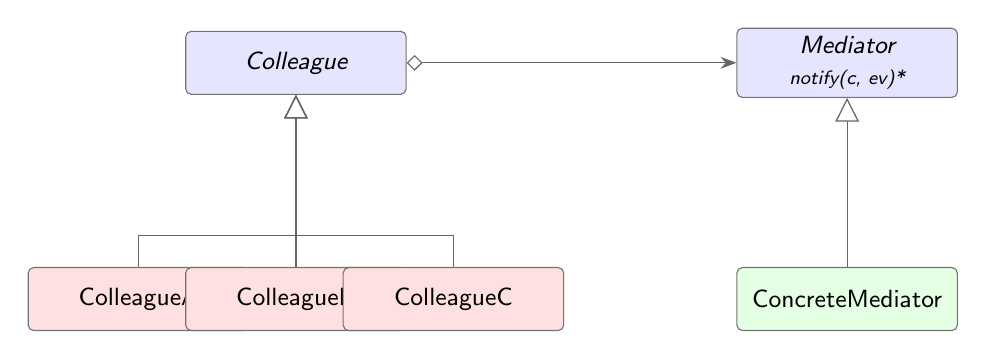
\begin{tikzpicture}[
  font=\sffamily\small,
  cls/.style={rectangle, rounded corners=2pt, draw=black!55, line width=0.4pt,
              minimum height=8mm, minimum width=28mm, inner sep=3pt, fill=white, align=center},
  abs/.style={cls, fill=blue!10, font=\sffamily\itshape\small},
  con/.style={cls, fill=red!12},
  imp/.style={cls, fill=green!10},
  inh/.style={-{Triangle[length=3mm,width=3mm,open]}, draw=black!60, line width=0.45pt},
  agg/.style={{Diamond[length=2mm,width=2mm,open]}-{Stealth[length=2mm]}, draw=black!60}
]
\node[abs] (med) at (4, 1.5) {Mediator \\ \scriptsize notify(c, ev)*};
\node[abs] (col) at (-3, 1.5){Colleague};
\node[con] (ca)  at (-5,-1.5){ColleagueA};
\node[con] (cb)  at (-3,-1.5){ColleagueB};
\node[con] (cc)  at (-1,-1.5){ColleagueC};
\node[imp] (cm)  at ( 4,-1.5){ConcreteMediator};

\draw[inh] (ca.north) -- ++(0,0.4) -| (col.south);
\draw[inh] (cb.north) -- (col.south);
\draw[inh] (cc.north) -- ++(0,0.4) -| (col.south);
\draw[inh] (cm.north) -- (med.south);
\draw[agg] (col.east) -- (med.west);
\end{tikzpicture}
\end{document}
